\documentclass[conference]{IEEEtran}
\IEEEoverridecommandlockouts
\usepackage[T1]{fontenc}
\usepackage[utf8]{inputenc}
\usepackage{amsmath,amssymb,amsthm,mathtools}
\usepackage{graphicx,booktabs,array,multirow,tabularx}
\usepackage{cite,url,enumitem}
\usepackage{microtype}
\usepackage{xcolor}
\usepackage{balance}
\usepackage{algorithm,algpseudocode}
\usepackage{stfloats}
\graphicspath{{figures/}}
\newtheorem{theorem}{Theorem}
\newtheorem{proposition}{Proposition}
\newtheorem{definition}{Definition}
\newcommand{\OO}{\mathcal{\Omega}}
\newcommand{\F}{\mathcal{F}}
\newcommand{\B}{\mathcal{B}}
\newcommand{\Q}{\mathsf{Q}}
\newcommand{\Sref}{\mathrm{S}}
\newcommand{\Gref}{\mathrm{G}}
\newcommand{\topk}{\operatorname{Top}\!\text{-}k}
\begin{document}
\title{Biological Findings That Survive Reannotation: Stable Query Processing Across Taxonomic Reference Systems}
\author{\IEEEauthorblockN{Adam Kiersztyn\IEEEauthorrefmark{1}, Magdalena Zo\l{}a\IEEEauthorrefmark{2}, Krystyna Kiersztyn\IEEEauthorrefmark{1}}
\IEEEauthorblockA{\IEEEauthorrefmark{1}Department of Computational Intelligence, Faculty of Mathematics and Information Technology,\\ Lublin University of Technology, Lublin, Poland}
\IEEEauthorblockA{\IEEEauthorrefmark{2}Department of Computer Science, Faculty of Electrical Engineering and Computer Science,\\ Lublin University of Technology, Lublin, Poland}
\IEEEauthorblockA{Corresponding author: Adam Kiersztyn (a.kiersztyn@pollub.pl).}}
\maketitle
\begin{abstract}
Scientific measurements can remain unchanged while the semantic reference used to interpret them evolves. Agreement between two complete annotations establishes only a pair of observations, not the persistence of a scientific claim under structured future revisions. We introduce \emph{budgeted semantic certificates}: a query operator returning a model-specific stability margin, an exact minimal edit budget required to violate a conclusion, and a constructive counterexample when violation is possible. A two-anchored uncertainty space contains both observed reference releases; edits may affect individual features, jointly switched blocks, or nested clades. For additive queries we derive exact worst-case margins using ordered block deltas and an exact min-plus hierarchy recurrence. We demonstrate the operator with 770 paired sequence features, 34 samples, 153,807 reads, and 2,097 taxonomic contrasts classified by SILVA 138 and Greengenes2 2024.09. Three agreed directional contrasts lose their guarantee after 1, 1, and 4 single-feature switches; a jointly evaluated top-1 ranking requires at least 44 such switches to admit an inversion. All 11 observed top-$k$ agreements are certified under a SILVA-family block model, compared with 10 under unrestricted independent feature switches. These different results are conditional on their respective, unvalidated biological coupling assumptions. An independent gut-to-soil validation extends the study to 41,328 identical sequence variants, 21,227,600 pooled reads, and SILVA~144 versus GTDB~r232. The leading phylum, \emph{Pseudomonadota}, remains certified under all independent binary assignments, with a minimum pairwise margin of 2,891,234 reads; in contrast, a two-feature witness reverses an initially agreed informative-genus top-one ranking. Exact enumeration validates the external operator in 1,320 cases. The resulting approach replaces a binary agreement judgment with an auditable \emph{distance to semantic failure}, while explicitly separating pooled-rank validity from biological inference.
\end{abstract}
\begin{IEEEkeywords}
taxonomic reannotation, semantic robustness radius, coupled uncertainty, certain answers, provenance, incremental view maintenance, microbiome
\end{IEEEkeywords}

\section{Introduction}
\label{sec:intro}
A scientific database is often treated as a stable record of measurements. Yet measurements are only one part of the interpretation embedded in a query. Reference tables, ontologies, taxonomic dictionaries, and annotation pipelines determine which measured entities contribute to a named aggregate. When those references evolve, the numerical input may be completely unchanged while the meaning of a returned answer is altered. This is not an exceptional condition of microbiome analysis; it is a general feature of data-intensive science in which measurement and interpretation follow different version histories.

Consider a longitudinal microbiome study. The read-count table is preserved, and each representative sequence retains its identifier. An initial classification maps a sequence to one genus; a later classifier, using a different taxonomy, maps the same sequence elsewhere. A conventional query engine is able to recompute a genus-level contrast for each reference version. It cannot infer from two coincident estimates whether the conclusion is immune to the class of annotation changes that the investigator considers admissible. Two answers are two observations, not a universal statement.

\emph{The central distinction of this paper is therefore between an observed agreement and a certified conclusion.} The first describes the outputs of particular releases. The second states a proposition that holds over every annotation configuration in an explicit feasible-world space. Both are useful, but they answer different questions. A scientifically responsible system must additionally distinguish such logical certainty from empirical support for the feasibility of the worlds themselves.

This observation suggests a change in the natural object of scientific query processing. Instead of returning only $\Q(D,R)$ for a database $D$ and reference version $R$, a query should be accompanied, when appropriate, by its \emph{semantic stability envelope}: the range of answers over a declared set $\OO$ of admissible reference interpretations, and a proof obligation associated with a specific claim. Such envelopes are properties of the query, the fixed measurement table, and the chosen space of interpretations. They are not probabilities, confidence intervals, or predictions of how future classifiers will behave.

The contribution is deliberately placed at the intersection of database semantics and scientific validation. Our primary statements are as follows:
\begin{enumerate}[leftmargin=*,nosep]
\item We represent alternative taxonomic assignments using unchanged sequence identifiers and fixed count denominators, and separate the two observed reference releases from broader, explicitly counterfactual reannotation spaces.
\item We introduce symmetric, two-anchored budgeted reannotation worlds, exactly compute the minimum number of coherent edits that can invalidate a directional or ranking claim, and return the violating assignment.
\item We demonstrate, on real paired-reference observations, three \emph{constructed sign-reversing witnesses} and one \emph{constructed ranking reversal} that expose the logical gap between observed agreement and certification.
\item We extend certificates to nested clade-edit events via exact min-plus tree messages, and benchmark indexed recertification against full recertification using the identical operator; neither standard dynamic programming nor generic IVM is claimed as newly invented.
\item We validate transferable ranking semantics on an independent gut-to-soil dataset of 41,328 paired sequence variants, showing both an all-world positive certificate and a two-edit genus inversion.
\item We provide a three-level evidence protocol: report the observed reference-specific outcomes, attach the model-conditional certificate and its margin, and state the independent biological assumptions and statistical evidence separately.
\end{enumerate}

The resulting framework is intended as a disciplined query layer, not as an automatic biomarker discovery system. We do not claim that counterfactual mixed annotations are necessarily plausible future classifier releases, nor do we claim that tree dynamic programming, sorting, or ordinary incremental maintenance are new primitives. The object of the guarantee is now accompanied by an exact \emph{distance to semantic failure}, enabling precise, query-specific stress tests under declared coherent edit models.

\section{Related Work and the Contribution Boundary}
\label{sec:related}
\subsection{Certain answers, provenance, and evolving reference data}
Classical incomplete-information databases separate recorded data from compatible completions \cite{imielinski1984}. Provenance semirings provide algebraic accounts of query dependence on input tuples \cite{green2007}, while probabilistic databases distinguish query evaluation under uncertainty from the use of materialized results \cite{dalvi2011}. Our reference alternatives can be viewed as a finite family of completions of an immutable observation table and an evolving taxonomic dimension. The present paper does not introduce a new semantics of incomplete information. It identifies a specific scientific contract---invariance of a directional or ranking claim---and makes its admissibility assumptions visible to the query user.

\subsection{Incremental computation}
Classical incremental view maintenance \cite{gupta1993,guptamumick1995,guptablakeley1995}, higher-order delta processing in DBToaster \cite{ahmad2012}, factorized maintenance in F-IVM \cite{kara2024}, and general stream-based incremental computation in DBSP \cite{budiu2023,budiu2025} provide powerful mechanisms for propagating updates to relational or analytical results. A derived certificate may be materialized or incrementally maintained using these principles. Our specialized update paths are consequently \emph{engineering demonstrations of a query semantics}, not evidence of general superiority to these systems. A production-grade, same-engine comparison remains future work.

\subsection{Microbiome reference evolution and inference}
QIIME 2 and its taxonomic-classification tools support reproducible amplicon workflows \cite{bolyen2019,bokulich2018}; SILVA and Greengenes2 are distinct reference resources \cite{quast2013,mcdonald2024}, and DADA2 provides high-resolution amplicon feature inference \cite{callahan2016}. Related ecosystem tools and workflows include phyloseq and Bioconductor pipelines \cite{mcmurdie2013,callahan2016workflow}. Interpretation also depends on sequencing modality: shotgun metagenomics has its own processing and reference assumptions \cite{quince2017}, while Greengenes2 explicitly seeks to bridge 16S and genome-derived taxonomic descriptions \cite{mcdonald2024}. Crucially, taxonomic label alignment is not the same as biological equivalence. Microbiome measurements are compositional \cite{aitchison1982,gloor2017}; abundance comparisons and repeated-measure effects require appropriate statistical models \cite{lin2020,lin2024,weiss2017,mcmurdie2014,knight2018}. A sign certificate for a fixed additive contrast is therefore not a hypothesis-test result and says nothing by itself about population-level inference.

\section{Fixed Measurements, Evolving Meaning}
\label{sec:model}
\subsection{Data model and the query contract}
Let $\F$ denote $n$ immutable sequence features and let $S$ denote samples. The read-count matrix $X=(x_{fs})$ is fixed, with sample totals $N_s=\sum_{f\in\F}x_{fs}>0$. Two complete reference annotations give taxonomic labels $a_f^{\Sref}$ and $a_f^{\Gref}$ for the same sequence identifier $f$. The reference-specific relational mapping $(f,r,a_f^r)$ must be versioned independently of $X$, so that a result can be traced to a specific pair of measurement and interpretation versions.

For a taxon label $t$ and sample $s$, the relative abundance in a world $\omega$ is
\begin{equation}
 A_{ts}(\omega)=\sum_{f\in\F}\frac{x_{fs}}{N_s}\,\mathbf{1}\{a_f^{\omega_f}=t\}.
 \label{eq:abundance}
\end{equation}
Fix a contrast between two prespecified sample groups through weights $w_s$, with $\sum_s w_s=0$; our empirical protocol uses subject-balanced within-site contrasts. The taxon contrast is
\begin{equation}
\begin{aligned}
\Q_t(\omega)&=\sum_s w_s A_{ts}(\omega)=\sum_{f\in\F}c_{ft}^{\omega_f},\\
c_{ft}^r&=\sum_s\frac{w_s x_{fs}}{N_s}\mathbf{1}\{a_f^r=t\}.
\end{aligned}
\label{eq:contrast}
\end{equation}
The second equality is decisive: with unchanged sample denominators and a fixed additive contrast, reference uncertainty acts through selectable feature contributions. It does not follow for arbitrary nonlinear diversity indices, estimated normalization factors, or statistical tests.

\subsection{A hierarchy of annotation worlds}
The \emph{observed} space $\OO_{\mathrm{obs}}$ contains exactly two complete assignments: all SILVA and all Greengenes2. The \emph{independent-feature} space $\OO_{\mathrm{feat}}=\{\Sref,\Gref\}^{\F}$ permits each feature to select one of its two measured assignments. A disjoint block partition $\B$ imposes a common selection for every feature within each block, yielding $\OO_{\B}$. In the experiment, we form family and phylum blocks from one anchor hierarchy (SILVA) to avoid crossing partitions. By construction,
\begin{equation}
\OO_{\mathrm{obs}}\subseteq\OO_{\mathrm{phylum}}\subseteq\OO_{\mathrm{family}}\subseteq\OO_{\mathrm{feat}}.
\label{eq:worldnest}
\end{equation}
This nesting is a property of the chosen stress-test representation, \emph{not} a discovered biological law. Coherent annotation releases are observed; the mixed worlds are mathematical alternatives. The data supply the two candidate labels per feature but do not supply a calibrated probability or a biological guarantee for independently choosing them.

\begin{definition}[Model-conditional claim certificate]
For query $\Q$ and a declared feasible-world set $\OO$, a directional conclusion is certified positive if $\Q(\omega)>0$ for every $\omega\in\OO$ and certified negative if $\Q(\omega)<0$ for every $\omega\in\OO$. A top-$k$ set $T$ is certified, under strict order, if $\Q_i(\omega)>\Q_j(\omega)$ for every $i\in T$, $j\notin T$, and $\omega\in\OO$. The certificate must identify $\OO$ and preserve a quantitative robustness margin.
\end{definition}

\noindent\textbf{A useful counterexample before the experiment.} Let three features contribute $(5,0)$, $(2,7)$, and $(0,4)$ under the two references. Their two complete-reference sums are 7 and 11. Independent reassignment gives the exact interval $[2,16]$. Thus even perfect knowledge of the two observed sums does not determine the space of permitted mixed-world answers. This toy example illustrates semantics only; the biological counterexamples appear in Sec.~\ref{sec:results}.

\section{Exact Certificates and Constructive Witnesses}
\label{sec:cert}
\subsection{Exact extrema for additive queries}
Write $c_{fq}^{r}$ for the additive contribution of feature $f$ to query $q$ under $r\in\{\Sref,\Gref\}$. The next statement yields the exact attainable extrema; intermediate values within the resulting interval need not themselves be attainable.

\begin{theorem}[Separable and block-coupled extrema]
For independent feature choices, the exact minimum and maximum are
\begin{equation}
 L_q^{\rm feat}=\sum_{f\in\F}\min_{r\in\{\Sref,\Gref\}}c_{fq}^{r},\quad
 U_q^{\rm feat}=\sum_{f\in\F}\max_{r\in\{\Sref,\Gref\}}c_{fq}^{r}.
\label{eq:boundfeat}
\end{equation}
For a disjoint block partition $\B$, let $C_{bq}^{r}=\sum_{f\in b}c_{fq}^{r}$. Then the exact bounds are
\begin{equation}
 L_q^{\B}=\sum_{b\in\B}\min_r C_{bq}^{r},\qquad
 U_q^{\B}=\sum_{b\in\B}\max_r C_{bq}^{r}.
\label{eq:boundblock}
\end{equation}
Both extrema are attained by explicit assignments of the feature or block choices.
\end{theorem}
\begin{IEEEproof}
For a fixed query, the objective is a sum of terms indexed by the independent choice units. There is no compatibility constraint between two distinct units. Choosing the smaller contribution in each unit achieves the lower bound, and choosing the larger contribution achieves the upper. Every feasible assignment has contributions at least the corresponding minima and at most the maxima. The singleton partition gives \eqref{eq:boundfeat}; general disjoint blocks give \eqref{eq:boundblock}.
\end{IEEEproof}

Consequently, $L_q>0$ certifies a positive direction and $U_q<0$ a negative one. A noncertified interval is not a biological observation of reversal. When the exact interval crosses zero \emph{strictly}, the extremizing assignments supply mathematical witnesses of opposite signs within $\OO$. Equality at zero is weaker and should not be labeled a strict sign reversal.

\begin{proposition}[Monotonicity under admissibility restrictions]
If $\OO_1\subseteq\OO_2$, then
$L_q(\OO_2)\le L_q(\OO_1)\le U_q(\OO_1)\le U_q(\OO_2)$.
\end{proposition}
\begin{IEEEproof}
The minimum over a superset cannot be larger than the minimum over its subset; the analogous maximum inequality follows by duality.
\end{IEEEproof}
A narrower interval obtained by choosing a smaller feasible space is a \emph{model change}; it is not, by itself, evidence that the new model better represents biology.

\subsection{From marginal intervals to exact ranking relations}
For a proposed descending top-$k$ set $T$, comparing $\min_{i\in T}L_i$ with $\max_{j\notin T}U_j$ supplies a familiar \emph{sufficient} test. It can be conservative because the two extrema may occur in different worlds. The correct joint object is the worst-case \emph{pairwise margin} under a shared world:
\begin{equation}
 m_{ij}(\OO)=\min_{\omega\in\OO}\big[\Q_i(\omega)-\Q_j(\omega)\big].
\label{eq:margin}
\end{equation}

\begin{theorem}[Exact pairwise certification for independent choices]
For an additive query family over $\OO_{\rm feat}$,
\begin{equation}
 m_{ij}^{\rm feat}=\sum_{f\in\F}\min\!\left(c_{fi}^{\Sref}-c_{fj}^{\Sref},\ c_{fi}^{\Gref}-c_{fj}^{\Gref}\right).
\label{eq:exactpair}
\end{equation}
The candidate set $T$ is the invariant strict top-$k$ set over $\OO_{\rm feat}$ if and only if $m_{ij}^{\rm feat}>0$ for all $i\in T$ and $j\notin T$. If any pairwise margin is negative, its feature-wise minimizing assignments construct a world in which an outside candidate outranks an inside one.
\end{theorem}
\begin{IEEEproof}
The difference $\Q_i-\Q_j$ is additive under the \emph{same} feature choices, so Theorem~1 applies to the contribution differences and yields \eqref{eq:exactpair}. Strict positivity of all cross-boundary differences is exactly the condition for unchanged top-$k$ membership. If a difference is negative, the attained minimizing world violates that order. A zero margin introduces possible ties and is not a strict certificate.
\end{IEEEproof}

The same construction applies to disjoint blocks after replacing feature contributions with block sums. Under cross-block dependencies, local minimization is generally not exact; a coupled optimizer or an appropriate dynamic program must respect those dependencies. The advance here is \emph{precision about the certification question}: the pairwise test exploits shared assignments rather than comparing unrelated marginal extremes. It should not be confused with a newly invented global ranking algorithm.

\subsection{Computing an explicit witness}
A scientific user benefits from a concrete counterexample rather than a binary ``not certified'' warning. For an observed positive contrast whose exact interval crosses zero, selecting $\arg\min_r c_{fq}^{r}$ at each feature gives a negative or zero minimizing world. For a negative observed contrast, use $\arg\max$. For top-$k$, choose the reference minimizing $c_{fi}^{r}-c_{fj}^{r}$ for the offending in/out pair. The feature IDs making different selections provide a traceable explanation of the formal failure. Witnesses are labeled \emph{constructed} in every output because they are combinations of observed per-feature assignments, not extra experimentally observed reference releases.


\section{Budgeted Semantic Robustness and Coherent Reannotation}
\label{sec:budget}
\subsection{The distance-to-failure question}
An uncertainty envelope that contains all independent feature choices gives a valid conditional guarantee, but may be too coarse to describe the effect of \emph{localized} reference evolution. Merely restricting all features of a family to change together is not a complete answer either: the restriction is a scientific assumption, and it leaves open how many coherent edits are needed before a claim becomes vulnerable. We therefore expose the \emph{edit model itself} as an explicit, auditable input to the query operator.

Consider a disjoint partition $\B=\{b_1,\ldots,b_G\}$ of the $770$ feature identifiers. The units can be singleton features or blocks derived from a declared anchor taxonomy. Each block must take its annotation consistently from one observed reference, while different blocks may select different references. Let $z_g\in\{0,1\}$ choose SILVA ($0$) or Greengenes2 ($1$). The two observed complete references correspond to $\mathbf 0$ and $\mathbf 1$. For edit budget $B$, define
\begin{equation}
\OO_B(\B)=\{\mathbf z:\min(\|\mathbf z\|_0,G-\|\mathbf z\|_0)\le B\}.
\label{eq:budgetworlds}
\end{equation}
Crucially, $\OO_0$ \emph{contains both complete references}; a one-sided ball centered only at SILVA could certify a result by excluding the observed Greengenes2 assignment. These spaces are nested, and for $B\ge\lfloor G/2\rfloor$ their union contains every block-consistent mixed world. A budget counts block selection changes \emph{relative to the nearer complete reference}; it is not a probabilistic estimate of likely taxonomy evolution.

For a query difference $q_i-q_j$, let $d_g^0=C_{gi}^{\Sref}-C_{gj}^{\Sref}$, $d_g^1=C_{gi}^{\Gref}-C_{gj}^{\Gref}$, and $\delta_g=d_g^1-d_g^0$. Put $D^a=\sum_g d_g^a$. Let $\delta_{(h)}^{\uparrow}$ and $\delta_{(h)}^{\downarrow}$ be the $h$-th smallest and largest changes, respectively.
\begin{theorem}[Exact two-anchored budget certificate]
For every additive query pair and the declared block partition, the worst shared-world margin over $\OO_B(\B)$ equals
\begin{align}
 m_{ij}(B)=\min\Big\{&D^0+\sum_{h=1}^{B'}\min(0,\delta_{(h)}^{\uparrow}),\notag\\
 &D^1-\sum_{h=1}^{B'}\max(0,\delta_{(h)}^{\downarrow})\Big\},
 \label{eq:budgetmargin}
\end{align}
where $B'=\min(B,G)$. A minimizing assignment can be constructed by switching exactly the selected most harmful blocks from the corresponding anchor. Once the deltas are formed, one margin and witness require $O(G\log G)$ time with ordinary sorting, or selection in linear expected time for a fixed budget.
\end{theorem}
\begin{IEEEproof}
Within the $B$-edit neighborhood of SILVA, choosing a switched block adds $\delta_g$ to $D^0$. No positive delta can improve a minimum, and the best permissible choices are the $B'$ smallest negative deltas. Within the $B$-edit neighborhood of Greengenes2, switching a block back to SILVA subtracts $\delta_g$ from $D^1$; the largest positive deltas are most harmful. The admissible space is the union of the two neighborhoods, so the global minimum is the smaller of their exact minima. The selected blocks attain each bound.
\end{IEEEproof}

This result applies to a single contrast by setting $q_j\equiv 0$, and to ranking preservation by taking a \emph{shared-world} difference between each selected taxon and every outside challenger. Let $T$ be an observed top-$k$ set. Its strict stability radius is the least $B$ such that some $i\in T$, $j\notin T$ satisfy $m_{ij}(B)\le0$; a negative margin yields a concrete inversion. Ties at zero are classified as \emph{uncertified strict ordering}, not necessarily as a reversal. For an agreed signed contrast $q$, orient its sign consistently under both anchors and define the same radius relative to $q-0$.
\begin{definition}[Semantic robustness radius]
The \emph{critical edit radius} $\rho(T,\B)$ is the smallest $B\in\{0,\ldots,G\}$ for which the prescribed strict certificate fails. Set $\rho=+\infty$ when every block-consistent world preserves the claim. The reported radius is always accompanied by the partition and versioned reference pair; it has no invariant meaning without them.
\end{definition}
For fixed partition and reference releases, the strict certificate is monotone in budget: its validity cannot recover after a larger budget has invalidated it. A budget-based certificate is therefore a compact explanation of \emph{how far} the guarantee extends, rather than a threshold tuned to obtain a desired answer.

\subsection{Nested clade events and exact tree semantics}
Taxonomic change may also affect nested rather than disjoint units. Let $H$ be a rooted, reference-anchored hierarchy. An event at node $v$ toggles the reference choice for every descendant feature, with nested events composing by exclusive-or. For a leaf feature $f$, its selected reference is $s\oplus\bigoplus_{v\in\operatorname{path}(f)} e_v$, where $s\in\{0,1\}$ denotes either observed anchor, $e_v\in\{0,1\}$ indicates an event, and $\sum_v e_v\le B$. This is an explicit \emph{clade-event scenario}, not a claim that classifier revisions literally operate by such toggles.

Let $M_v(s,b)$ be the minimum aggregate contribution below node $v$ for an incoming state $s$ and exactly $b$ events in that subtree. For an internal node with children $u_1,\ldots,u_m$,
\begin{equation}
 M_v(s,b)=\min_{e\in\{0,1\}}\min_{\substack{\sum_j b_j=b-e\\b_j\ge0}}
 \sum_j M_{u_j}(s\oplus e,b_j).
 \label{eq:treebudget}
\end{equation}
At a leaf, $M_f(s,0)=d_f^s$ and $M_f(s,1)=d_f^{1-s}$, with all infeasible states infinite. The exact global margin is $\min_{s\in\{0,1\},\,b\le B}M_{\rm root}(s,b)$.
\begin{proposition}[Soundness and cost of clade-event messages]
The recurrence in \eqref{eq:treebudget} computes exact minima under the stated parity and event-budget semantics. For a tree with $|V|$ nodes and maximum budget $B$, straightforward min-plus child convolution takes $O(|V|B^2)$ time and $O(|V|B)$ materialized state; a local contribution change affects only the ancestor messages of its leaf, though recomputation cost depends on their degrees and stored convolution state.
\end{proposition}
\begin{IEEEproof}
A leaf has precisely the stated two event options. At an internal node, every feasible configuration uniquely specifies its local event $e$ and a budget allocation among the children; conditioned on the outgoing parity, the children's contributions are additive and independent. Taking the minimum over these choices gives the exact optimum by induction. Each edge combines two arrays of length $B+1$ through a min-plus convolution, giving the stated worst-case cost for the straightforward algorithm.
\end{IEEEproof}
The recurrence is \emph{standard tree dynamic programming}. The methodological contribution is the auditable, two-anchored, edit-budgeted \emph{certificate contract} and its query-relative robustness radius; we do not claim invention of min-plus convolution or generic incremental maintenance \cite{kara2024,budiu2023}.

\section{Incremental Maintenance and Reannotation Transactions}
\label{sec:updates}
A reference upgrade is naturally a transaction on a versioned annotation relation. The system retains the previous mapping, checks that the feature keys remain aligned, records the new release and its provenance, determines the affected query dependencies, and updates the certificate state. This transaction should never silently rewrite the scientific measurement matrix.

For a disjoint block $b$ and query $q$, an update changes its two stored candidate contributions from $(C_{bq}^{\Sref},C_{bq}^{\Gref})$ to $(\widetilde C_{bq}^{\Sref},\widetilde C_{bq}^{\Gref})$. With an inverted index from blocks to affected queries, the exact lower-bound update is
\begin{equation}
\Delta L_q=\min_r\widetilde C_{bq}^{r}-\min_r C_{bq}^{r},
\quad \Delta U_q=\max_r\widetilde C_{bq}^{r}-\max_r C_{bq}^{r}.
\label{eq:delta}
\end{equation}
The arithmetic is proportional to the number of affected $(b,q)$ pairs, excluding indexing, preprocessing and materialization costs. Pairwise top-$k$ margins can likewise be maintained from per-feature or block difference contributions, although their storage and update cost depends on how many candidate pairs are materialized.

For explicitly tree-coupled choices, a bottom-up min/max dynamic program propagates allowable parent--child states. A local edit only requires recomputing affected ancestor-path messages. For tree height $h$, at most $K$ states per node, and $Q$ maintained queries, a simple bound for affected-path work is $O(hK^2Q)$; exact constants depend on sparsity and compatible transitions. This is \emph{standard tree dynamic programming}. We test eager path maintenance, deferred (lazy) evaluation and full recomputation to characterize workload regimes, not to claim a novel IVM algorithm.

The decision to maintain certificates eagerly or lazily has a systems implication. Eager maintenance buys immediate read availability by paying at every annotation update. Lazy maintenance defers invalidations and may be preferable when reads are relatively rare. The consistency model, caching strategy, and memory budget are part of a production design; the Python prototype does not settle these engineering choices.

\subsection{A certificate-aware query interface}
The proposed interface separates a \emph{data answer} from a \emph{claim answer}. A data answer is the aggregate under a named observed reference. A claim answer is a tuple
\begin{equation}
\mathsf{Cert}(q,v,\OO)=\big(\Q_q^v,L_q(\OO),U_q(\OO),\gamma_q,\sigma_q\big),
\label{eq:record}
\end{equation}
where $v$ identifies the currently observed release, $\gamma_q$ is the strict margin to the decision boundary, and $\sigma_q$ records the applicable status. For positive directional claims, $\gamma_q=L_q$; for negative claims, $\gamma_q=-U_q$. A ranking claim stores the smallest exact cross-boundary pairwise margin. The certificate also requires a separate provenance record identifying the immutable feature table, both mapping versions, normalization, weight construction, feasibility constraints and executable derivation of its witness. Without these identifiers the same numeric interval can be mistakenly reused under a changed query or sample normalization.

The distinction implies a concrete governance rule. A reannotation transaction invalidates a certificate whenever the set of possible feature contributions or admissibility rules changes, even when the current observed aggregate happens to be unchanged. In contrast, a change to metadata that does not affect the query dependency graph need not force recomputation. This is a natural application of provenance-based dependency tracking rather than a new transaction algorithm. The advantage of a certificate-aware interface is epistemic: it prevents a cached numerical answer from silently standing in for a different scientific proposition.

\subsection{Computational state and worst-case bookkeeping}
Under independent switches, storing the two contributions for every affected feature--query pair requires space proportional to the number of nonzero dependencies, plus $O(Q)$ aggregate bounds. A sparse inverted index maps a revised feature to those queries it may influence. If an update changes $d_f$ such pairs, the bound-arithmetic part of processing that update is $O(d_f)$. An exact top-$k$ certificate over a supplied set $T$ and candidate universe $C$ has $k(|C|-k)$ cross-boundary comparisons. Keeping a margin summary for every candidate pair can be expensive when $|C|$ is large; on-demand pairwise evaluation or a restricted candidate neighborhood trades memory for query latency. These ordinary resource trade-offs are part of the supported operator's scope, and no unmeasured constant-time guarantee is implied.

The block case stores one pair of alternative contributions per affected block--query pair. Its arithmetic update cost is proportional to the number of affected pairs, but block recomputation may require revisiting member features unless their contributions are separately maintained. A coupled tree may require message tables with $O(K^2)$ compatibility work per affected edge and query. Consequently, a biological claim may be inexpensive to certify algebraically while the administrative cost of maintaining trustworthy version and lineage metadata is non-negligible. The latter must be included in a future end-to-end system comparison.

\section{Experimental Design and Reproducibility}
\label{sec:exp}
\subsection{Real data and query construction}
We use the public QIIME~2 \emph{Moving Pictures} example dataset \cite{bolyen2019} as an intentionally transparent methodological substrate. The frozen table contains 770 shared representative-sequence features, 34 samples, 153,807 reads and two participants. The identical sequence IDs were classified using SILVA~138 and Greengenes2~2024.09. Thus the count matrix, sample-depth denominators and feature identities remain fixed. Only taxonomy lookup assignments vary. The work does not constitute an independent population-scale validation or a confirmatory clinical study.

We consider three anatomical-site contrasts (gut minus tongue, left palm minus right palm, gut minus left palm) at phylum, family and genus levels. This yields nine contexts and 2,097 additive taxon-contrast queries. Three $k$ choices ($1,3,5$) over the nine contexts yield 27 top-$k$ scenarios. Classification labels are compared literally except for the documented Proteobacteria/Pseudomonadota normalization; we do not infer arbitrary synonym correspondences from similar taxon strings. The original per-subject weighting and unmodified denominators are retained.

\subsection{Correctness and system tests}
The empirical pipeline regenerates its original five stage-25 outputs byte-for-byte, including contrasts, top-$k$ summaries and validation metadata. A separate exhaustive suite compares algebraic bounds with enumeration on small constructed spaces and checks monotonicity under disjoint-block coupling. Its 1,440 comparisons include 720 block-nesting checks. We evaluate exact pairwise ranking margins for the 11 observed-agreement settings and generate witness assignments when strict certification fails. Source-level update studies compare specialized indexed updates, vectorized recomputation and a measured batched SQL/DuckDB execution path. Separate synthetic-tree trials use identical feasible-world semantics across path updates, lazy messages and full tree dynamic programming. These are distinct workloads and their performance ratios must not be pooled.

For biological interpretation, the key validity gates are identical feature identifiers and fixed read totals. A prior 62-sample rodent export was excluded because its two reference tables lacked a verified feature-ID correspondence and common denominators. For genuine external validation we instead use a separate gut-to-soil QIIME~2 visualization \cite{caporaso2026dual,meilander2024data}: 41,328 unique ASV identifiers paired under SILVA~144 and GTDB~r232, sharing the same pooled per-ASV frequency vector (21,227,600 total reads). This second study tests taxon-abundance \emph{rankings}, not cross-group abundance contrasts: the released visualization exposes pooled frequencies and the number of samples containing each feature, but not the per-sample count matrix. Both studies retain exactly the same feature keys and denominators \emph{within} each reference pair; their taxonomic vocabularies are not otherwise assumed equivalent.

\section{Results: When Agreement Does Not Certify Stability}
\label{sec:results}
\subsection{Taxonomic change is heterogeneous}
Label agreement differs strongly by rank and weighting. In the observed two-reference audit, literal read-weighted agreement is 58.27\% for phyla, 78.93\% for families, and 28.13\% for genera. Among SILVA-defined blocks with at least two features, heterogeneous changed/unchanged literal genus status occurs in 9 of 20 phyla and 44 of 78 families. These measurements invalidate an easy inference that taxonomic families tend to switch as indivisible units; forced block coupling must be treated as a sensitivity assumption.

\begin{figure}[t]
\centering
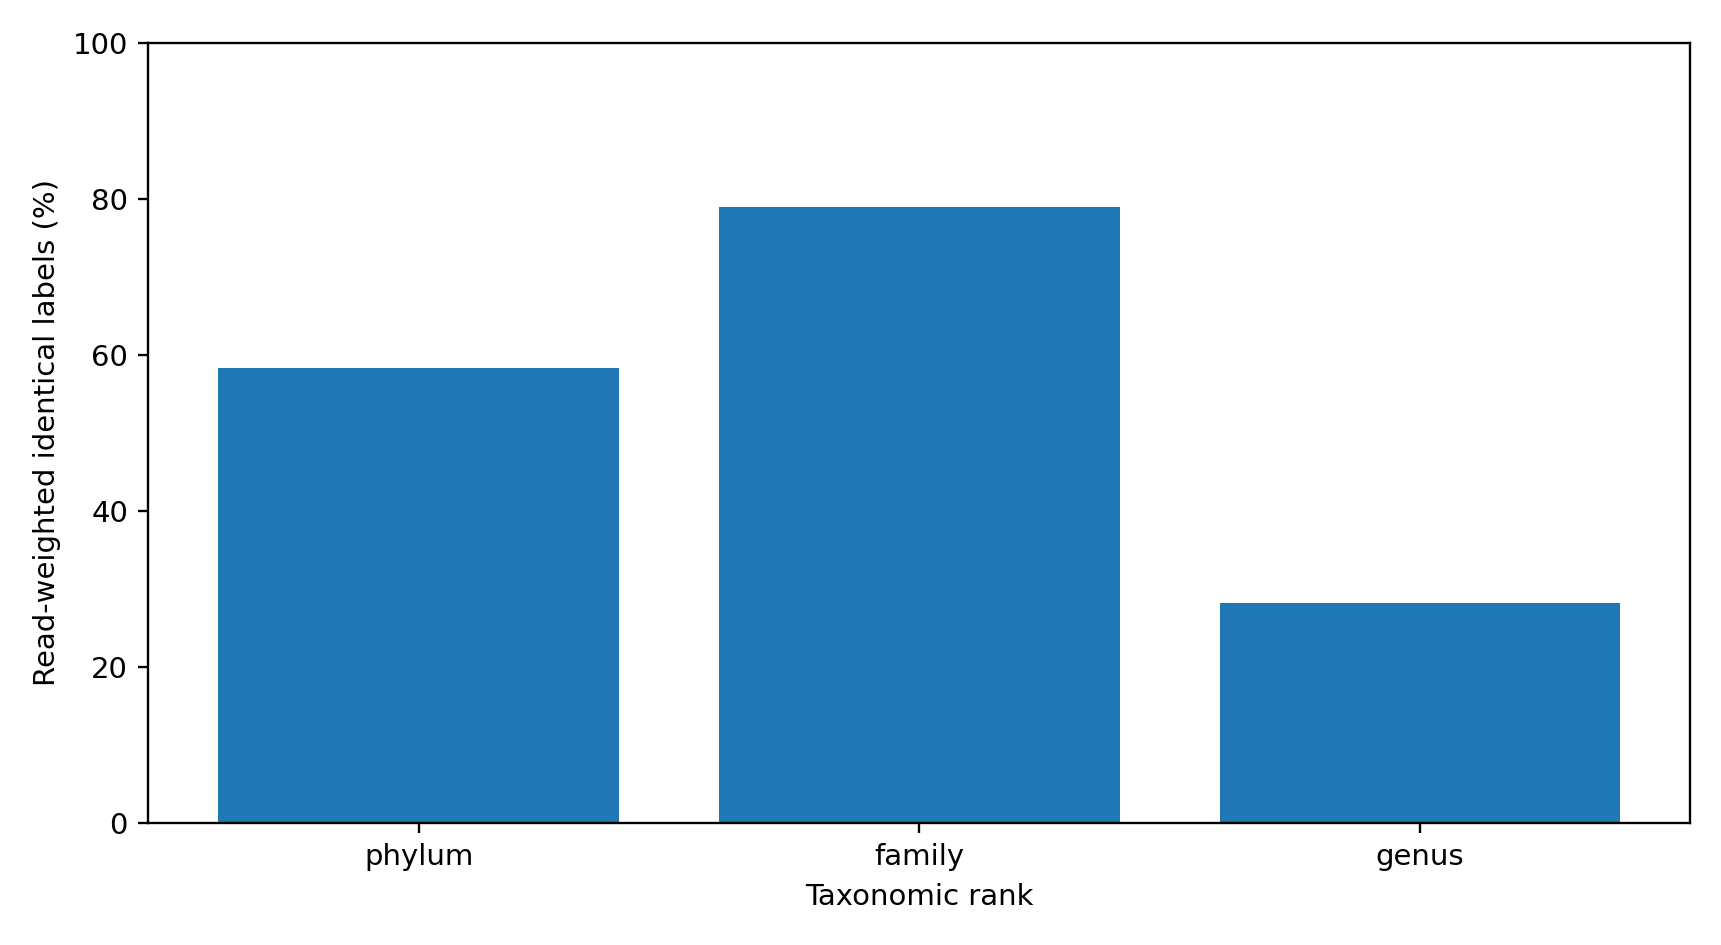
\includegraphics[width=.94\columnwidth]{old1.png}
\caption{Measured read-weighted literal taxonomic label agreement across two classifiers applied to the same sequences. Ranks use the stated conservative normalization; the figure does not validate biological synonymy or taxonomic correctness.}
\label{fig:agreement}
\end{figure}

The profile in Fig.~\ref{fig:agreement} reveals why a single aggregate ``taxonomy agreement'' percentage would be inadequate. Agreement is substantially higher at the family level than at the genus level, while rank changes and different nomenclature conventions can affect a scientifically visible query in different ways. The query-relative certificate is therefore intentionally calculated after all feature-specific contributions have been instantiated: it is the scientific question, not a global reference score, that determines which annotation disagreements matter. A low overall label agreement does not imply a failed conclusion, and high label agreement does not establish a certificate.

\begin{table}[t]
\centering
\caption{Real paired-reference experiment and independent correctness tests. A certificate is conditional on the indicated feasible-world space.}
\label{tab:design}
\small
\begin{tabular}{@{}lr@{}}
\toprule
Quantity & Observed value\\\midrule
Samples / aligned features / reads & 34 / 770 / 153,807\\
Observed full-reference versions & 2\\
Contrasts / rank--site contexts & 2,097 / 9\\
Top-$k$ contexts / observed agreements & 27 / 11\\
Certified observed top-$k$ agreements & 10\\
Exactly constructed sign reversals & 3\\
Exact pairwise tests & 3,860\\
Exhaustive bound tests & 1,440\\
Maximum bound error & $1.78\times10^{-15}$\\
\bottomrule
\end{tabular}
\end{table}

\subsection{Three sign reversals beyond the two observed worlds}
Across the 2,097 contrast queries, 394 have the same nonzero direction in both observed reference versions (summing the observed-agreement counts in the nine contexts). Three of these 394 are not direction-certified under independent feature choices. More importantly, the exact extremizing assignments in all three cases produce \emph{strictly opposite} signs. This replaces the ambiguous statement ``the interval includes zero'' with reproducible, feature-level witnesses.

\begin{table}[t]
\centering
\caption{Three exact sign-reversing witnesses, left palm minus right palm. Values are percentage points; the mixed world is constructed, not observed.}
\label{tab:witness}
\footnotesize
\begin{tabular}{@{}lrrr@{}}
\toprule
Taxon (rank) & SILVA & Greengenes2 & Mixed\\\midrule
Aerococcaceae (F) & $-0.0071$ & $-0.2187$ & $+0.0193$\\
Corynebacterium (G) & $+0.2459$ & $+0.6047$ & $-0.3976$\\
Prevotella (G) & $+0.2765$ & $+1.6298$ & $-0.0117$\\
\bottomrule
\end{tabular}
\vspace{2pt}
\parbox{\columnwidth}{\footnotesize F: family; G: genus. The extremizing configurations select the Greengenes2 assignment for 1, 4 and 5 of the 770 features, respectively.}
\end{table}

\begin{figure*}[t]
\centering
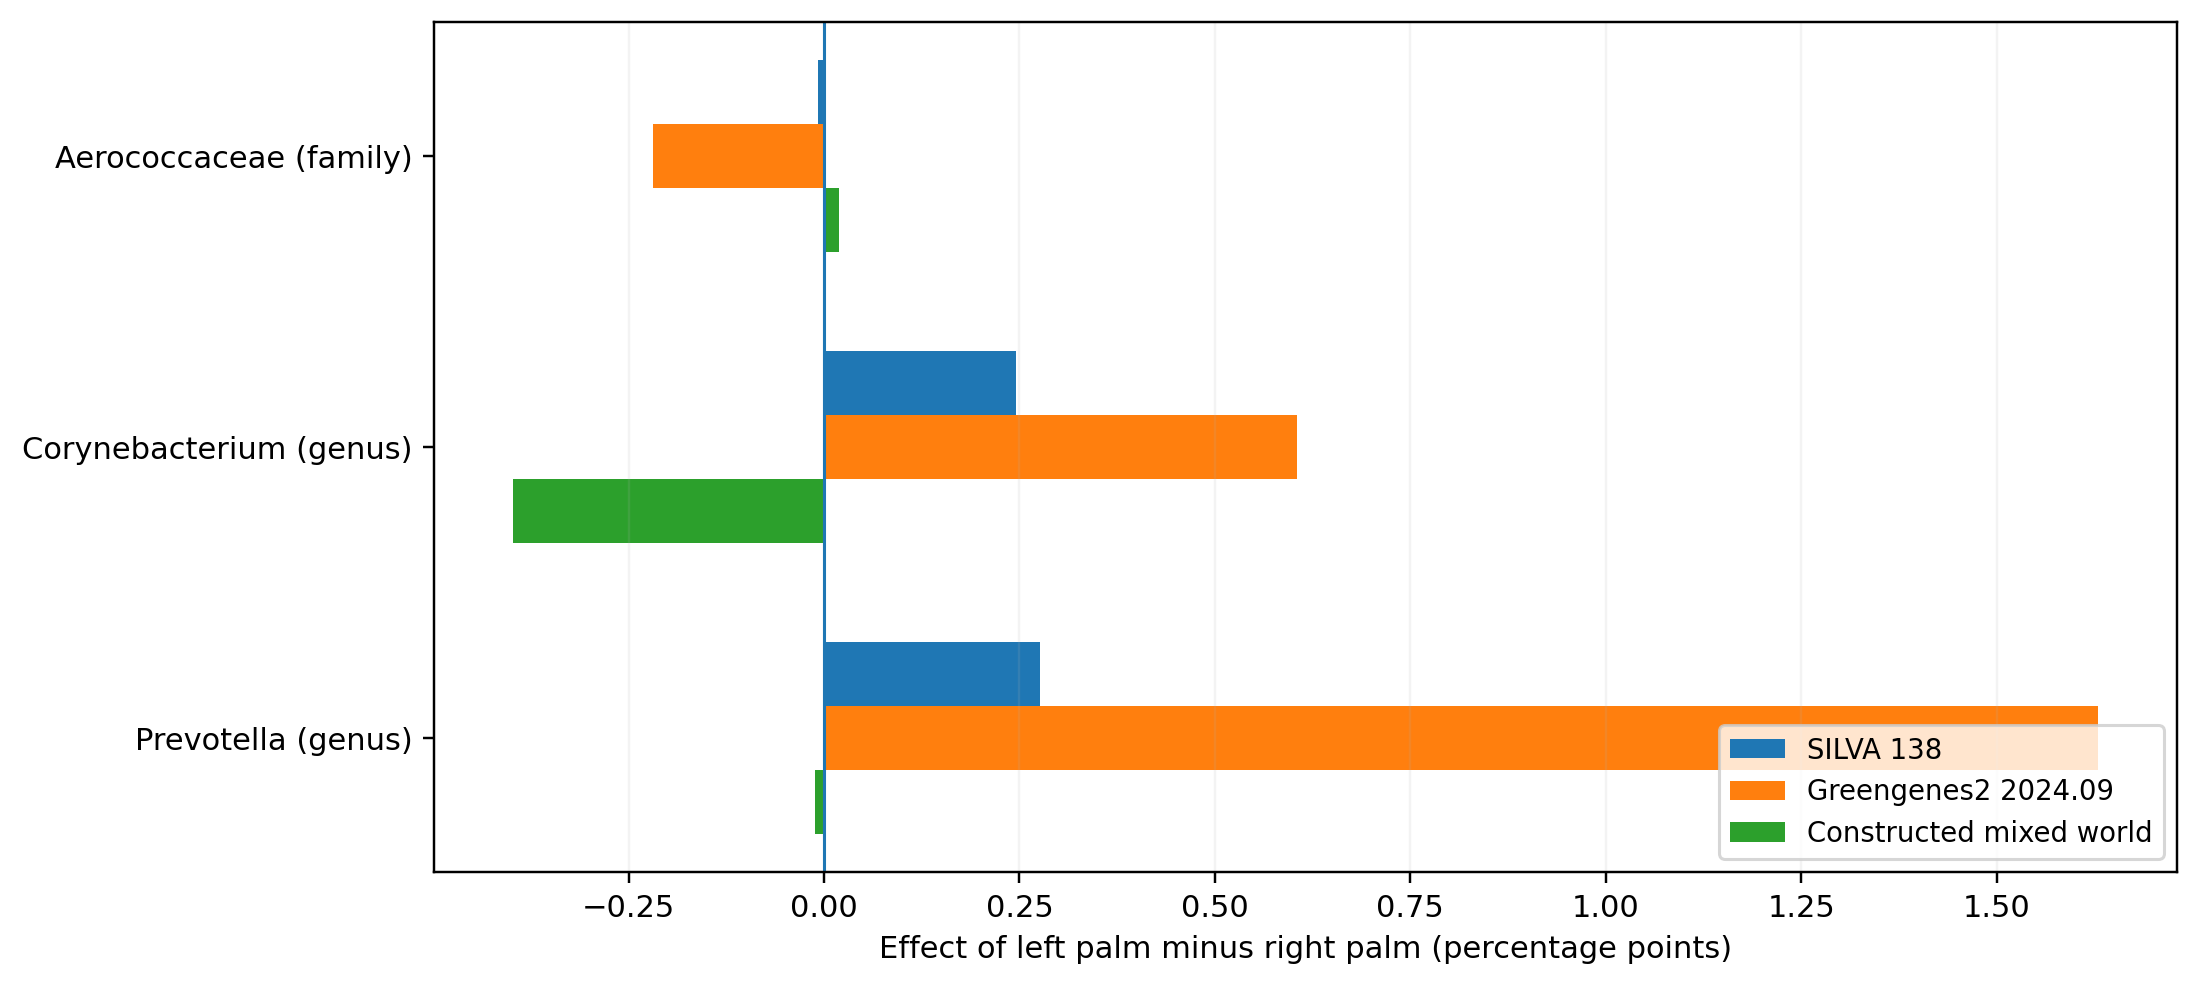
\includegraphics[width=.82\textwidth]{actual_sign_reversals.png}
\caption{The meaning of agreement depends on the admissible-world model. All three taxon contrasts have matching signs under the two complete reference releases, but a precisely constructed feature-independent mixed world reverses each direction. These are model-conditional mathematical counterexamples, not observed biological reversals or statistically significant findings.}
\label{fig:witness}
\end{figure*}

Fig.~\ref{fig:witness} and Table~\ref{tab:witness} show the same computed contrasts on a scale of percentage points. The small number of counterexamples is not a prevalence estimate for microbiome reannotation; the dataset contains only two people and two reference versions. The result demonstrates the logical separation of sampled agreement and universal certification.

\subsection{A ranking witness and an exact pairwise test}
The 27 rank--site--$k$ scenarios yield 11 cases in which the two complete references return the same top-$k$ set. Ten are certified by the sufficient interval test. The exact shared-world pairwise analysis considers 3,860 comparisons and also certifies 10 of 11. It therefore provides \emph{no additional positive certifications} on this dataset. Its empirical value is instead diagnostic: the sole noncertified observed agreement admits a concrete ranking inversion.

In the left-palm versus right-palm phylum-level top-1 context, \emph{Pseudomonadota} is ranked first under both complete references. An exact feature-independent worst-case assignment produces a pairwise margin of $-0.00521511$ (relative-abundance contrast units), allowing \emph{Firmicutes} to overtake it. This is not an artifact of combining separate score intervals: both candidates are evaluated in the \emph{same constructed world}. The negative margin witnesses a failure of invariance under $\OO_{\rm feat}$, not evidence of an actual historical reannotation effect.

\begin{figure*}[t]
\centering
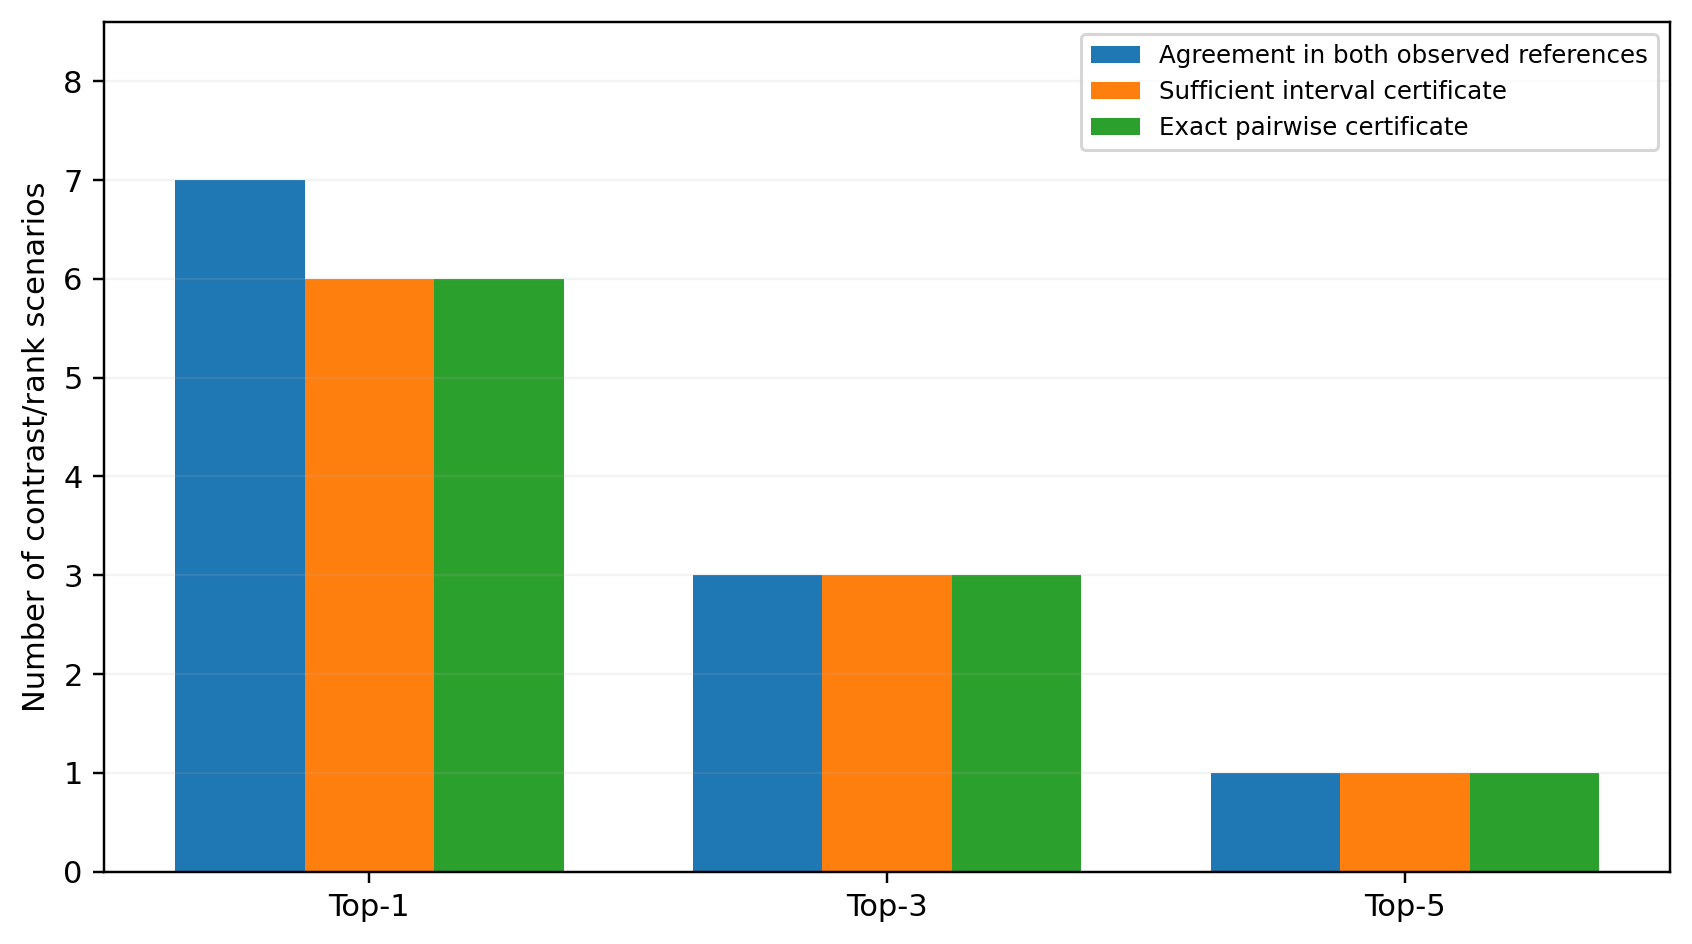
\includegraphics[width=.73\textwidth]{actual_topk_certificates.png}
\caption{Observed top-$k$ agreements, conservative interval certificates, and exact shared-world pairwise certificates over the 27 tested scenarios. The exact pairwise test does not increase the number of positive certifications (10/11 observed agreements), but its negative top-1 result admits an explicit constructed ranking-reversal witness.}
\label{fig:topk}
\end{figure*}

\subsection{Correctness of finite-world and update computations}
All 1,440 exhaustive finite-world comparisons passed. The maximum absolute gap between enumerated extrema and algebraic endpoints was $1.78\times10^{-15}$; all 720 nested-block monotonicity checks passed. An additional 80 exhaustive small-tree tests passed with maximum error $3.55\times10^{-15}$. In the matched-semantics update experiments, eager, lazy and full recomputation returned the same certificate values. Reproduction of the original five biological stage-25 outputs was byte-for-byte exact. These checks validate implementation correctness for tested models; they do not validate the biological probability of any counterfactual world.

\subsection{Incremental computation: benefit and boundary}
In the real 2,097-query Windows workload, median update latencies were $0.00633\,$ms for the indexed specialized update, $0.01582\,$ms for vectorized affected-query recomputation, and $2.30038\,$ms for the tested Python-invoked DuckDB batch path. The first comparison offers relevant evidence of reduced arithmetic within the tested implementation; the large DuckDB ratio mainly characterizes this particular invocation and SQL execution path. It is \emph{not} a fair claim of superiority over optimized native DuckDB IVM, F-IVM or DBSP.

Separate same-semantics synthetic-tree experiments further illuminate update/read frequency. Table~\ref{tab:perf} reports the latest repeated total-time measurements across 120 changes per run and three repetitions. At 1,023 nodes with certificate reads after every 20 updates, lazy maintenance was faster than eager maintenance, while eager had a small advantage for every-update reads. The full-rebuild baseline is substantially more expensive when every update is followed by a read, yet the advantage narrows as reads become rarer. This is a \emph{workload-dependent trade-off}, not a universally optimal policy.

\begin{table}[t]
\centering
\caption{Matched-semantics synthetic-tree benchmark: median total runtime (ms), 120 updates, 3 repeats. ``Every $r$'' denotes certificate-read frequency.}
\label{tab:perf}
\footnotesize
\begin{tabular}{@{}rrrrr@{}}
\toprule
Nodes & Every $r$ & Eager & Lazy & Rebuild\\\midrule
255 & 1 & 31.75 & 34.07 & 546.65\\
255 & 5 & 26.21 & 19.74 & 107.92\\
255 & 20 & 27.81 & 11.45 & 27.01\\
1023 & 1 & 39.11 & 43.48 & 2410.75\\
1023 & 5 & 37.91 & 28.30 & 452.96\\
1023 & 20 & 34.08 & 19.93 & 115.71\\
\bottomrule
\end{tabular}
\end{table}

\begin{figure}[t]
\centering
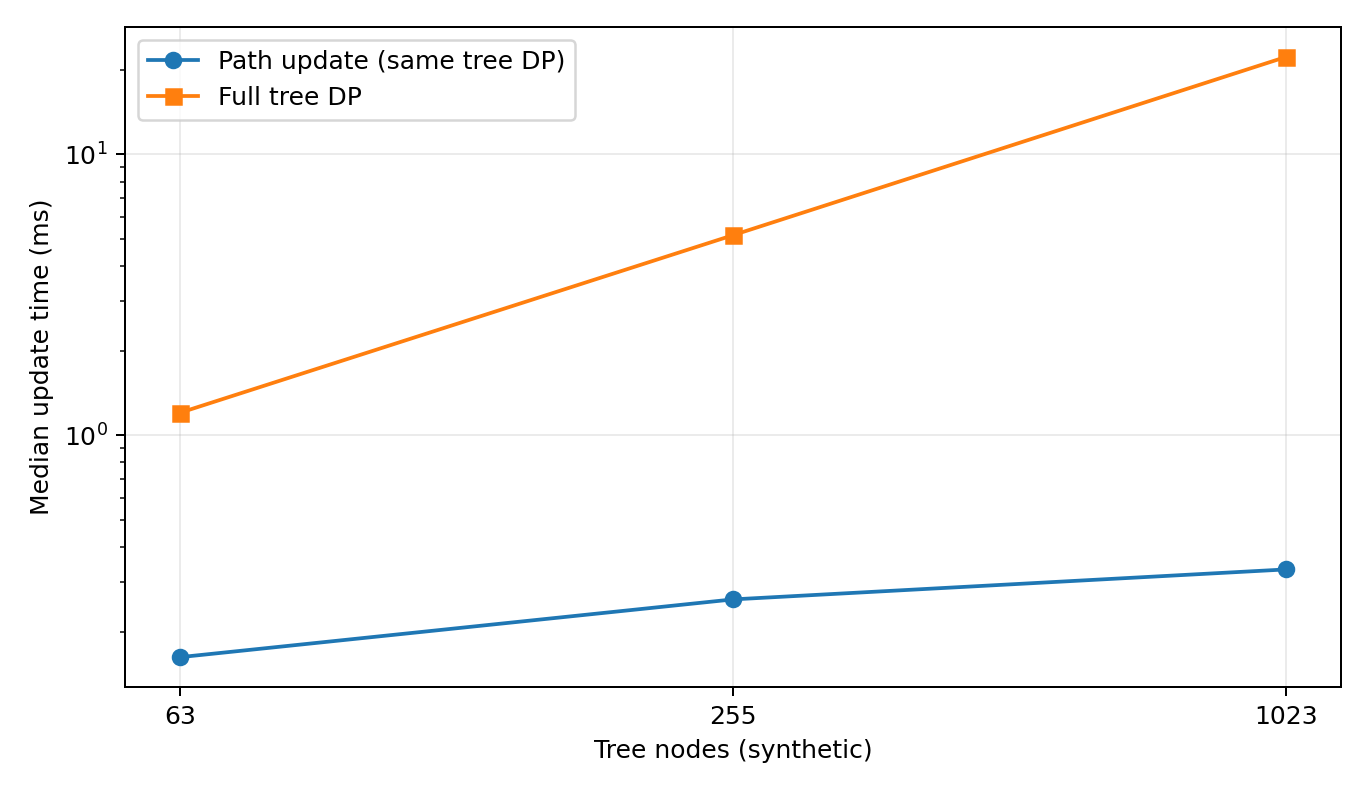
\includegraphics[width=.99\columnwidth]{old4.png}
\caption{A separate matched-semantics synthetic-tree experiment: median time for path-only recomputation and full tree dynamic programming as tree size grows. The comparison does not use biologically learned transition constraints.}
\label{fig:tree}
\end{figure}

The experimentally useful systems question is therefore not whether delta updates are categorically faster, but \emph{which certificate state should be materialized under an observed update/read schedule}. The formal guarantees remain the same while the materialization policy changes. As with the certificate itself, the trade-off is best reported together with its assumptions.


\section{Additional Results: The Geometry of Semantic Failure}
\label{sec:budgetresults}
\subsection{Exact critical edit radii on paired microbiome features}
We recomputed all 27 top-$k$ scenarios and 394 two-reference, same-sign taxon contrasts on the original 770 features with both versioned assignments. Three partition models yielded 770 singleton units, 206 SILVA-family units, and 40 SILVA-phylum units. Blank family/phyla labels were \emph{not} merged into artificial shared ``unknown'' blocks: missing labels received feature-specific fallback units. Thus the hierarchy is a transparent anchor-derived sensitivity model, not an independently validated correspondence between taxonomic systems.

For the three previously identified sign failures under singleton choices, the exact critical radii are 1 for \emph{Aerococcaceae}, 1 for \emph{Corynebacterium}, and 4 for \emph{Prevotella}. The top-1 \emph{Pseudomonadota} versus \emph{Firmicutes} order remains protected for all budgets up to 43 singleton changes and becomes falsifiable at exactly \emph{44} switches from one observed complete reference. The $B=44$ minimizer has a strictly negative margin, hence supplies an actual ranking-inversion witness \emph{within the declared scenario}. No mixture was seen as an observed third classifier release.

\begin{figure}[t]
\centering
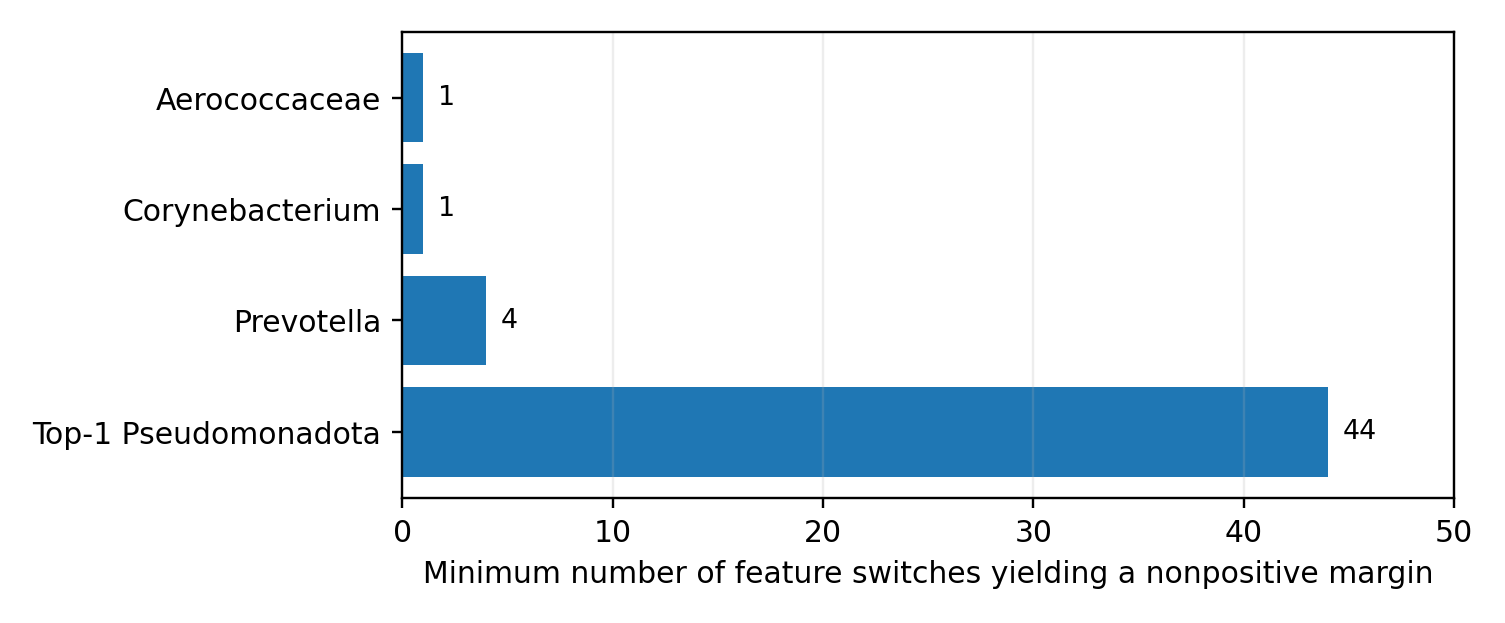
\includegraphics[width=\columnwidth]{fig_robustness_radii.png}
\caption{New real-data results: minimal numbers of independent feature switches needed for a nonpositive margin. These are distances to mathematical counterexamples, not probabilities of biological change.}
\label{fig:radii}
\end{figure}

\begin{table}[t]
\centering
\caption{Real-data, model-conditional robustness under two-anchored switching. All 11 agreed observed top-$k$ scenarios are considered in every row.}
\label{tab:frontier}
\footnotesize
\begin{tabular}{@{}lrrrr@{}}\toprule
Model & Units & $B=0$ & $B=16$ & Full world\\\midrule
Features & 770 & 11 & 11 & 10\\
SILVA family & 206 & 11 & 11 & 11\\
SILVA phylum & 40 & 11 & 11 & 11\\
\bottomrule\end{tabular}
\end{table}

Table~\ref{tab:frontier} and Fig.~\ref{fig:frontier} reveal an important asymmetry: a block-coherent model can maintain all eleven exact rankings even though the feature-independent model admits a real arithmetic counterexample. That apparent improvement \emph{cannot} be interpreted as additional biological evidence. It reflects a smaller, explicitly assumed space of reannotation worlds. For the 394 observed same-sign contrasts, the numbers with a constructed opposite-or-zero-sign world are 3 under singleton choices, 1 under SILVA-family blocks, and 0 under SILVA-phylum blocks. These counts come from the present small dataset; they are not population rates.

\begin{figure}[t]
\centering
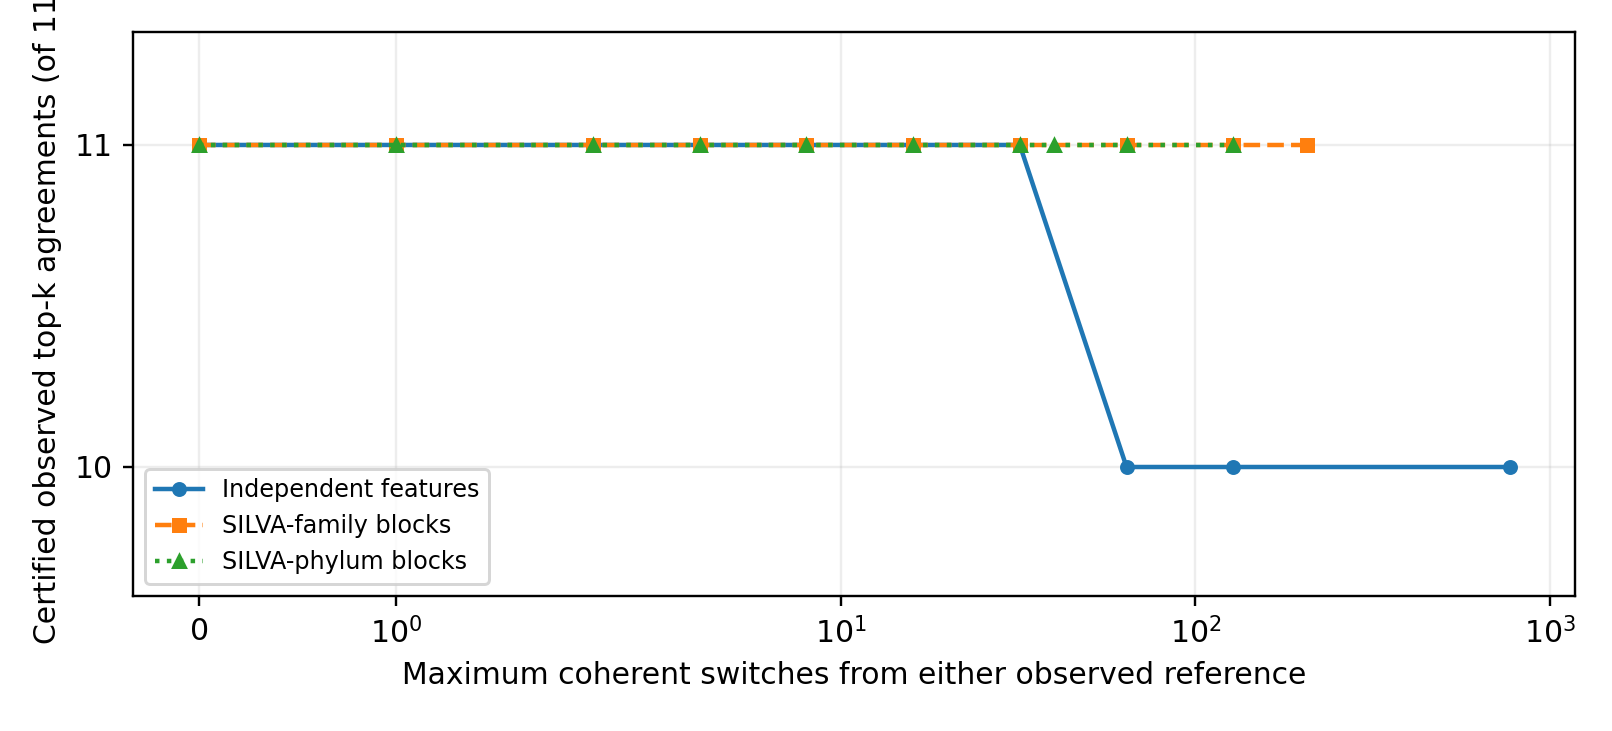
\includegraphics[width=\columnwidth]{fig_budgeted_frontier.png}
\caption{New real-data certificate frontiers as the maximum number of coherent reference switches increases. Each model contains both complete observed references; curves are conditional on different partition assumptions.}
\label{fig:frontier}
\end{figure}

\subsection{Tree-coupled checks and equal-operator maintenance}
A SILVA-anchored tree with 1,528 nodes was constructed from the paired feature identifiers and available phylum, family, and genus hierarchy. Exactly computed min-plus margins for four representative query differences over budgets zero through four include a negative sign witness for \emph{Aerococcaceae} at one clade event, for \emph{Corynebacterium} at one event, and for \emph{Prevotella} at four events; the examined \emph{Pseudomonadota}/\emph{Firmicutes} comparison retained a positive margin for budgets up to four. This is a limited proof-of-concept sample, not a full-tree evaluation of all 2,097 queries.

We checked the new two-anchor block solver with 2,970 exhaustive small-world cases (maximum absolute error $3.55\times10^{-15}$), plus 1,380 exhaustively enumerated random-tree cases (maximum $8.88\times10^{-16}$). Every tested optimizer matched enumeration. To avoid comparing different query semantics, we also implemented two variants of the \emph{same exact budgeted pairwise operator} in Python: full recertification of all $240$ candidate--challenger pairs after each update, versus recertification only of pairs affected by an updated taxon payload. On a synthetic aggregate-payload workload with 206 groups, 64 taxa, top-$4$, budget four, 120 updates and three repetitions, median total times were $959.8$ and $25.1$ ms respectively (median per-run speed ratio $37.3$), with zero numerical discrepancy. This comparison is an implementation-level index benefit; it is \emph{not} a comparison against an optimized, native F-IVM, DBSP, or database engine.

\begin{figure}[t]
\centering
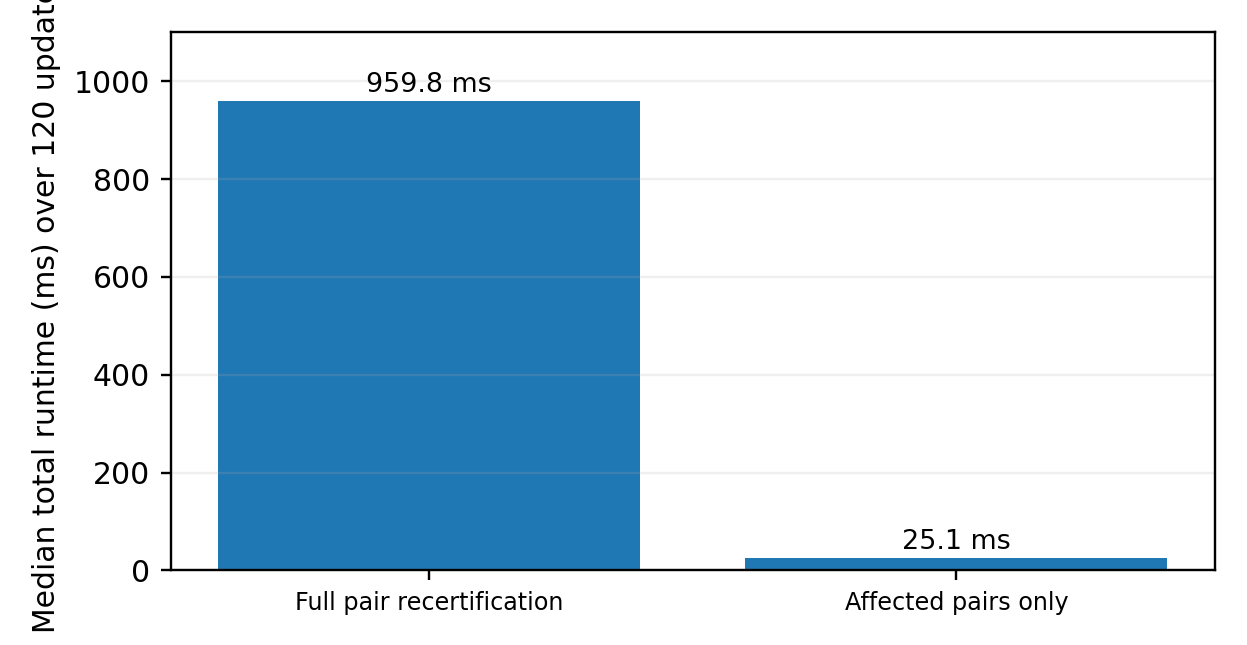
\includegraphics[width=.98\columnwidth]{fig_same_semantics.png}
\caption{New same-operator Python benchmark: median end-to-end runtime for 120 synthetic aggregate-payload updates, with exact agreement between full and affected-pair recertification. Not a native database-system comparison.}
\label{fig:sameop}
\end{figure}

\subsection{Interpretive limits and systems implications}
There are now two separable questions for evaluation: whether a certificate is \emph{algorithmically exact for its world model}, and whether its world model is an independently defensible description of reannotation. The former is supported by the enumerations and constructive witnesses; the latter is not proven by regrouping SILVA labels. Nor does a large synthetic maintenance ratio imply a systems breakthrough over mature IVM. The independent second cohort reported next provides external validation of paired-key rankings and certificates, but not an empirical law of allowable family-coupled reannotation, population-level inference, or a production-engine comparison.


\section{Independent Biological Validation: From Concordance to Certificates}
\label{sec:external}
\subsection{A second cohort and a different reference pair}
A method claiming to maintain scientific meaning across reference updates should not depend on one particular set of taxonomic dictionaries. We therefore evaluated the same ranking certificate on the independent public \emph{gut-to-soil} amplicon data, whose paired QIIME~2 visualization reports SILVA~144 and GTDB~r232 classifications for \textbf{41,328 identical amplicon sequence variants} (ASVs) \cite{caporaso2026dual,meilander2024data}. The two columns share one pooled frequency vector totaling \textbf{21,227,600 reads}; the experiment changes only taxonomic assignments and never refits its denominator. This yields an auditable paired-key comparison even though the biological samples, reference versions, and taxonomic labeling conventions differ from the \emph{Moving Pictures} experiment.

Unlike the primary dataset, the public tabulation used here does not expose the per-sample abundance matrix. The supported query class is therefore \emph{pooled taxon-count top-$k$}, not phenotype contrasts or participant-level inference. We treat missing ranks as unassigned rather than imputing a shared ``unknown'' taxon and report literal label agreement separately from any biological equivalence claim. When forming SILVA-family edit blocks, an ASV lacking a SILVA family receives its own fallback block; the resulting partition has 2,928 distinct edit units.

\subsection{Reference agreement depends on query resolution}
On the shared count vector, two nonempty literal annotations agree for 17,377,393 reads (\textbf{81.86\%}) at phylum level, 9,528,607 (\textbf{44.89\%}) at family level and 5,669,841 (\textbf{26.71\%}) at genus level (Fig.~\ref{fig:external_agreement}). These proportions are measured against the common 21,227,600-read denominator; absent labels and nonidentical nomenclature contribute to the remainder. Thus higher agreement at a coarse rank cannot be extrapolated to the finer query whose conclusion the scientist actually uses.

\begin{figure}[t]
\centering
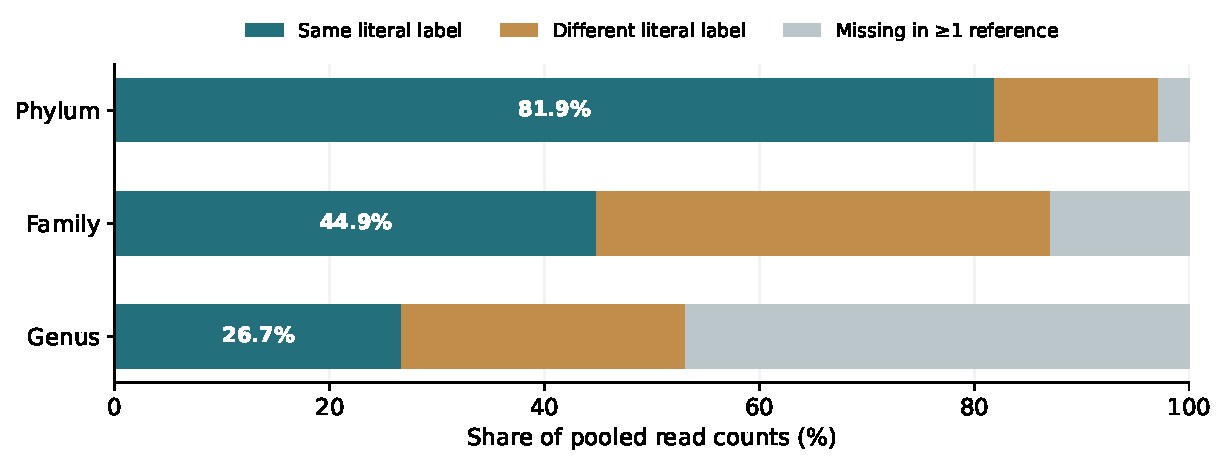
\includegraphics[width=.98\columnwidth]{Fig_external_1_taxonomic_agreement.pdf}
\caption{Independent data: identical nonempty literal labels as shares of the \emph{same} 21,227,600 pooled reads under SILVA~144 and GTDB~r232. Label identity is not independently validated ontological equivalence.}
\label{fig:external_agreement}
\end{figure}

\subsection{A certified winner and a two-edit counterexample}
Both complete reference assignments place \emph{Pseudomonadota} first among 116 literal phylum labels. Importantly, the stronger universal claim is also true \emph{within the specified world model}: exact pairwise minimization against all 115 alternative labels has a minimum margin of \textbf{2,891,234 reads} (13.62\% of the shared denominator), even with unrestricted independent switching between the two annotations of every ASV (Fig.~\ref{fig:external_margins}). Consequently, the top-one conclusion has an unbounded finite edit radius within this binary-choice model. The observed top-three and top-five sets, by contrast, differ between the reference versions and therefore cannot be certified for any model containing both complete assignments.

At genus resolution the interpretation is different. After \emph{consistently excluding} noninformative genus names (including \texttt{Incertae\_Sedis}, \texttt{uncultured}, and generic ``other'' suffixes), both observed classifications rank \emph{Rhodococcus} first. Its strict advantage over competitor \emph{Rhodanobacter}, however, has a critical two-ASV edit radius from the GTDB anchor. The pairwise worst-case margin is +75,129 pooled reads at budget zero, +3,874 after one switch, and \textbf{--2,293 after two switches}. The two documented feature identifiers contribute 71,255 and 6,167 reads under their SILVA alternatives. Thus the two-reference consensus is insufficient to certify this rank, and a concrete violating assignment can be inspected rather than merely inferred from overlapping intervals. Under the more restrictive SILVA-family switching assumption, the same top-one result remains strictly certified. Family-wise coherence is a modeling choice, not an empirically established mechanism of future reannotation (Fig.~\ref{fig:external_margins}).

\begin{figure}[t]
\centering
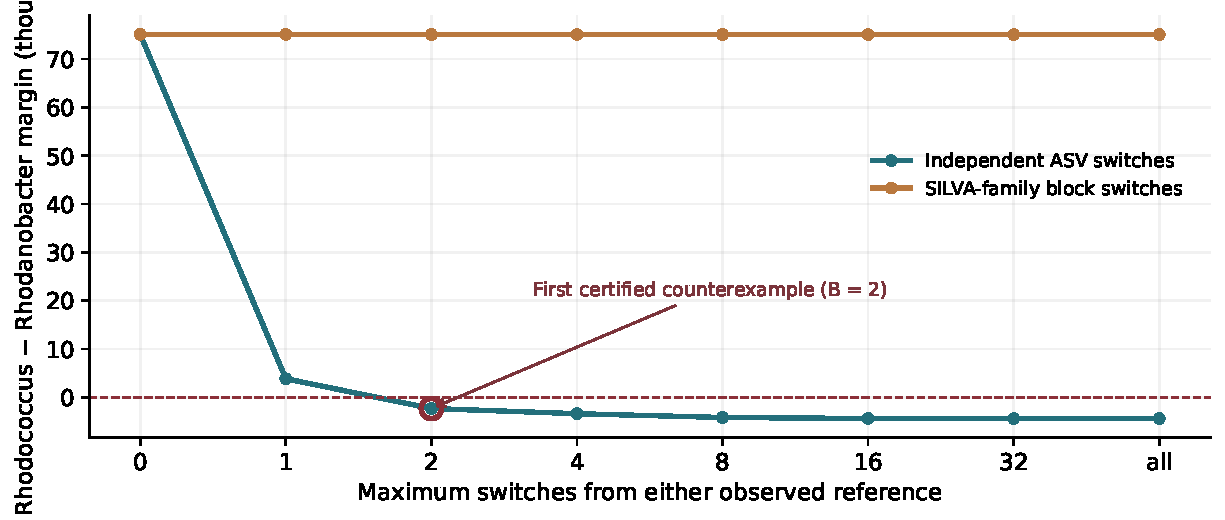
\includegraphics[width=.98\columnwidth]{Fig_external_3_genus_witness.pdf}
\caption{Independent data: exact genus pairwise margin under two-anchored ASV edit budgets, showing the constructive two-edit inversion after filtering noninformative genus labels. The whole-family assumption yields a different certificate.}
\label{fig:external_margins}
\end{figure}

\subsection{Reproduction and validity boundary}
The implementation checked uniqueness of all 41,328 feature identifiers, nonnegative integral counts, a common frequency denominator, and pairwise margins for all phylum competitors. On \textbf{1,320} independent small-world enumeration tests, optimized budgeted margins matched exhaustive enumeration to maximum absolute error $8.88\times10^{-16}$. Source identifiers, script, derived tables, QIIME~2 artifact SHA-256, and the witness ASV keys are retained in a separate reproduction package. The source visualization is linked rather than redistributed.

This experiment substantially strengthens the case for \emph{cross-reference computational transfer}: it reproduces both logical outcomes, a provably stable winner and a constructive instability, on a far larger and independent ASV domain. It does not validate the biological plausibility of counterfactual mixed releases or the accuracy of genus-level synonymy; nor does it convert pooled rank comparisons into phenotypic, clinical or causal conclusions.

\section{Discussion: A Granular View of Scientific Reliability}
\label{sec:discussion}
\subsection{Three noninterchangeable layers of evidence}
The interpretation of a scientific query may evolve at three distinct levels. First, \emph{observational concordance} compares a finite set of known complete annotations. Second, \emph{model-conditional certification} proves a property throughout a declared family of alternative annotations. Third, \emph{scientific validity} assesses whether the alternative family and the target contrast represent a biologically meaningful question, with suitable replication and statistical inference. A strong result at one level does not subsume the others.

This separation has practical consequences for how systems should report results. An output record should contain $(\Q^{\Sref},\Q^{\Gref})$, the certificate interval or pairwise margin, the admissibility-model identifier, feature-level provenance sufficient to inspect a witness, and a clear semantic status. We distinguish \emph{certified}, \emph{observationally concordant but not certified}, and \emph{observationally discordant}. Importantly, an uncertified query is not automatically unstable in reality; only an exact constructed witness proves noninvariance \emph{within the chosen model}.

\subsection{What the experiments do not establish}
The feature-independent model is intentionally permissive: it includes combinations that may never occur in an internally coherent taxonomic release. Family and phylum coupling restrict that space but are not biologically established by two observed references. Indeed, mixed changed/unchanged patterns within actual family and phylum groups caution against treating block switches as empirical laws. In a separate audit of 703 simple count queries, the family-block assumption tightened only one interval; imposing a new constraint is not synonymous with obtaining informative narrower answers.

Taxonomic nomenclature introduces another limitation. Greengenes2 and SILVA may use different clade resolutions, suffixes and names for biologically related but nonidentical categories. We use conservative literal matching except for the explicit Proteobacteria/Pseudomonadota normalization; no global cross-reference synonymy is assumed. A genus-level sign contrast can consequently represent a different biological entity in the two references unless a scientifically justified crosswalk is supplied.

Nor does directional robustness imply a statistically reliable biomarker. Relative abundances have compositional constraints; the small 34-sample, two-participant \emph{Moving Pictures} dataset is a methodological demonstration and does not support population-level generalizations. The experimental 10,000--100,000-query scaling workloads replicate templates; they test systems behavior and do not add independent biological observations. The separate gut-to-soil experiment passed the identifier-alignment and fixed-count gate for pooled rankings; it could not validate group-specific microbiome contrasts or the likelihood of counterfactual family-block switches. Finally, our Python/NumPy paths do not establish parity or superiority against production-grade incremental database engines.

\subsection{Where the conceptual step leads}
A useful next-generation scientific database should preserve, as versioned first-class data, not only the original measurements but also the evolving reference mappings, allowable transformations, and the \emph{claims that depend on them}. Such an infrastructure can maintain a scientific conclusion as a computable object with a query lineage, a declared semantic uncertainty model and a measurable margin to failure. Granularity then plays two roles: it determines how the interpretation space is partitioned, and it determines how much of a maintained query state requires revision when a reference mapping changes.

The present work identifies a precise boundary between what can already be guaranteed and what remains open. Exact certificates are available for additive queries with separable or block-coupled choices; exact pairwise ranking constraints use the same principle. More expressive nonlinear queries, empirically calibrated dependencies across taxonomic assignments, and large-scale same-engine incremental benchmarks remain genuine research tasks. These are not cosmetic extensions: each changes either the feasible space, the supported claim language, or the cost of producing a scientific guarantee.

\subsection{A falsifiable validation agenda}
The independent second cohort supplies a stable feature-key domain and a distinct observed pair of classifiers. A stronger follow-up would obtain longitudinally released, expert-harmonized taxonomies and test whether empirically grounded feasibility constraints exclude implausible mixed worlds without discarding realistic transitions. Such a design would distinguish the \emph{soundness of a mathematical bound for its specified space} from the \emph{coverage of real reference changes by that space}. A second essential step is to embed the same certificate expression in a mature IVM engine and report matched-semantics latency distributions, memory, preprocessing costs, storage layout and transaction boundaries. These requirements define measurable hypotheses rather than relying on a qualitative expectation that incremental computation should be faster.

A complementary test involves uncertainty at multiple granularities. A singleton feature is a fine-grained choice unit; a family block is a coarser one; a whole-reference switch is coarser still. Under nested partitions the extrema obey the monotonicity property of Sec.~\ref{sec:cert}, but the \emph{scientific appropriateness} of each granularity must be assessed independently. This is the principal granular insight of the work: tightening the feasible space changes the logical strength of a certificate only when the coupling has defensible provenance. An interval made narrow by an unvalidated grouping is more visually appealing but not more trustworthy.

\section{Conclusion}
The durability of a scientific conclusion is not determined solely by the durability of its measurements. When reference systems evolve, query answers acquire an additional source of uncertainty: the possibility that an unchanged observation is interpreted through a different semantic map. We have formalized that uncertainty as an explicit family of annotation worlds, derived exact certificates for an additive query class, and demonstrated how certificate state can be maintained as reference assignments change.

The empirical lesson is constructive. Across a small, fully paired public microbiome dataset, two complete taxonomic releases can agree on a direction or top-$k$ set while precisely constructed mixed-reference worlds overturn it. The three sign-reversing witnesses and one top-$1$ inversion make this logical distinction observable; exhaustive tests confirm the mathematical implementation, while update experiments clarify its computational costs. Their force is semantic, not clinical: the witnesses prove model-conditional noninvariance, not the biological likelihood of such reannotations.

Scientific databases can therefore report a more meaningful object than a point estimate or a binary agreement flag: \emph{an answer, a declared interpretation space, and an auditable proof of the claim that survives that space}. On an independent 41,328-ASV dataset, the same operator additionally certifies universal top-one dominance at phylum level and finds a two-feature counterexample for an agreed genus-level winner. The next step is to calibrate the biological plausibility of allowable assignment worlds across longitudinal reference releases and to implement the operators in mature database engines. Until then, explicit limits are not a weakness of certification---they are part of what makes a certificate scientifically interpretable.

\section*{Reproducibility and Data Availability}
The real-data inputs are derived from the public QIIME~2 \emph{Moving Pictures} tutorial, with paired SILVA~138 and Greengenes2~2024.09 classifications of the same 770 features. The validated local package records immutable feature counts, versioned assignments, five reproduced stage-25 outputs, exact witness tables, tests and scripts. An additional public gut-to-soil paired-taxonomy visualization provides 41,328 aligned ASVs under SILVA~144 and GTDB~r232; our separately versioned script and derived result tables reproduce the pooled top-$k$ certificate analysis. The exact original QIIME~2 visualization (SHA-256: \texttt{e8aa584032374072c3b8607a870fadd1}\allowbreak\texttt{79bd9c6e5198d37f605c71fcddb03cfb}) is linked, not redistributed. Primary-data validation and external pooled-rank validation are distinct experiments. Public release of the final integrated reproduction package is pending the authors' approval and redistribution audit. Funding support should be stated only after author confirmation.

\section*{Acknowledgement}
This work was supported by the Lublin University of Technology Scientific Fund, grant FD-20/IT-3/002. The final funding line and all author metadata are subject to approval by the authors.

\section*{AI-Generated Content Acknowledgement}
OpenAI ChatGPT assisted with language drafting, editing, code development, analysis, and figure preparation in the Introduction, Formal Methods, Experiments, Results, and Discussion. The named authors retain responsibility for the scientific hypotheses, verification of data and sources, correctness of code, interpretation of results, and all claims. This disclosure requires final author approval before submission.

\begin{thebibliography}{27}
\bibitem{green2007} T. J. Green, G. Karvounarakis, and V. Tannen, ``Provenance Semirings,'' in \emph{Proc. ACM PODS}, 2007, pp. 31--40, doi: 10.1145/1265530.1265535.
\bibitem{ahmad2012} Y. Ahmad, O. Kennedy, C. Koch, and M. Nikolic, ``DBToaster: Higher-order Delta Processing for Dynamic, Frequently Fresh Views,'' \emph{Proc. VLDB Endow.}, vol. 5, no. 10, pp. 968--979, 2012, doi: 10.14778/2336664.2336670.
\bibitem{kara2024} A. Kara, M. Nikolic, D. Olteanu, and H. Zhang, ``F-IVM: Analytics over Relational Databases under Updates,'' \emph{VLDB J.}, vol. 33, pp. 903--929, 2024, doi: 10.1007/s00778-023-00817-w.
\bibitem{bolyen2019} E. Bolyen \emph{et al.}, ``Reproducible, Interactive, Scalable and Extensible Microbiome Data Science Using QIIME 2,'' \emph{Nat. Biotechnol.}, vol. 37, pp. 852--857, 2019, doi: 10.1038/s41587-019-0209-9.
\bibitem{quast2013} C. Quast \emph{et al.}, ``The SILVA Ribosomal RNA Gene Database Project: Improved Data Processing and Web-Based Tools,'' \emph{Nucleic Acids Res.}, vol. 41, pp. D590--D596, 2013, doi: 10.1093/nar/gks1219.
\bibitem{budiu2023} M. Budiu, T. Chajed, F. McSherry, L. Ryzhyk, and V. Tannen, ``DBSP: Automatic Incremental View Maintenance for Rich Query Languages,'' \emph{Proc. VLDB Endow.}, vol. 16, no. 7, pp. 1601--1614, 2023, doi: 10.14778/3587136.3587137.
\bibitem{budiu2025} M. Budiu \emph{et al.}, ``DBSP: Automatic Incremental View Maintenance for Rich Query Languages,'' \emph{VLDB J.}, vol. 34, art. 39, 2025, doi: 10.1007/s00778-025-00922-y.
\bibitem{callahan2016} B. J. Callahan \emph{et al.}, ``DADA2: High-Resolution Sample Inference from Illumina Amplicon Data,'' \emph{Nat. Methods}, vol. 13, pp. 581--583, 2016, doi: 10.1038/nmeth.3869.
\bibitem{mcdonald2024} D. McDonald \emph{et al.}, ``Greengenes2 Unifies Microbial Data in a Single Reference Tree,'' \emph{Nat. Biotechnol.}, vol. 42, pp. 715--718, 2024, doi: 10.1038/s41587-023-01845-1.
\bibitem{lin2020} H. Lin and S. D. Peddada, ``Analysis of Compositions of Microbiomes with Bias Correction,'' \emph{Nat. Commun.}, vol. 11, art. 3514, 2020, doi: 10.1038/s41467-020-17041-7.
\bibitem{dalvi2011} N. Dalvi, C. R\'e, and D. Suciu, ``Queries and Materialized Views on Probabilistic Databases,'' \emph{J. Comput. Syst. Sci.}, vol. 77, no. 3, pp. 473--490, 2011, doi: 10.1016/j.jcss.2010.04.006.
\bibitem{gupta1993} A. Gupta, I. S. Mumick, and V. S. Subrahmanian, ``Maintaining Views Incrementally,'' \emph{ACM SIGMOD Rec.}, vol. 22, no. 2, pp. 157--166, 1993, doi: 10.1145/170036.170066.
\bibitem{guptamumick1995} A. Gupta and I. S. Mumick, ``Maintenance of Materialized Views: Problems, Techniques, and Applications,'' \emph{IEEE Data Eng. Bull.}, vol. 18, no. 2, pp. 3--18, 1995.
\bibitem{guptablakeley1995} A. Gupta and J. A. Blakeley, ``Using Partial Information to Update Materialized Views,'' \emph{Inf. Syst.}, vol. 20, no. 8, pp. 641--662, 1995, doi: 10.1016/0306-4379(95)00035-6.
\bibitem{imielinski1984} T. Imieli\'nski and W. Lipski, Jr., ``Incomplete Information in Relational Databases,'' \emph{J. ACM}, vol. 31, no. 4, pp. 761--791, 1984, doi: 10.1145/1634.1886.
\bibitem{bokulich2018} N. A. Bokulich \emph{et al.}, ``Optimizing Taxonomic Classification of Marker-Gene Amplicon Sequences with QIIME 2's q2-feature-classifier Plugin,'' \emph{Microbiome}, vol. 6, art. 90, 2018, doi: 10.1186/s40168-018-0470-z.
\bibitem{mcmurdie2013} P. J. McMurdie and S. Holmes, ``phyloseq: An R Package for Reproducible Interactive Analysis and Graphics of Microbiome Census Data,'' \emph{PLoS ONE}, vol. 8, no. 4, e61217, 2013, doi: 10.1371/journal.pone.0061217.
\bibitem{gloor2017} G. B. Gloor, J. M. Macklaim, V. Pawlowsky-Glahn, and J. J. Egozcue, ``Microbiome Datasets Are Compositional: And This Is Not Optional,'' \emph{Front. Microbiol.}, vol. 8, art. 2224, 2017, doi: 10.3389/fmicb.2017.02224.
\bibitem{aitchison1982} J. Aitchison, ``The Statistical Analysis of Compositional Data,'' \emph{J. R. Stat. Soc. Ser. B}, vol. 44, no. 2, pp. 139--160, 1982, doi: 10.1111/j.2517-6161.1982.tb01195.x.
\bibitem{callahan2016workflow} B. J. Callahan, K. Sankaran, J. A. Fukuyama, P. J. McMurdie, and S. P. Holmes, ``Bioconductor Workflow for Microbiome Data Analysis: From Raw Reads to Community Analyses,'' \emph{F1000Research}, vol. 5, art. 1492, 2016, doi: 10.12688/f1000research.8986.2.
\bibitem{quince2017} C. Quince, A. W. Walker, J. T. Simpson, N. J. Loman, and N. Segata, ``Shotgun Metagenomics, From Sampling to Analysis,'' \emph{Nat. Biotechnol.}, vol. 35, pp. 833--844, 2017, doi: 10.1038/nbt.3935.
\bibitem{lin2024} H. Lin and S. D. Peddada, ``Multigroup Analysis of Compositions of Microbiomes with Covariate Adjustments and Repeated Measures,'' \emph{Nat. Methods}, vol. 21, pp. 83--91, 2024, doi: 10.1038/s41592-023-02092-7.
\bibitem{mcmurdie2014} P. J. McMurdie and S. Holmes, ``Waste Not, Want Not: Why Rarefying Microbiome Data Is Inadmissible,'' \emph{PLoS Comput. Biol.}, vol. 10, no. 4, e1003531, 2014, doi: 10.1371/journal.pcbi.1003531.
\bibitem{knight2018} R. Knight \emph{et al.}, ``Best Practices for Analysing Microbiomes,'' \emph{Nat. Rev. Microbiol.}, vol. 16, pp. 410--422, 2018, doi: 10.1038/s41579-018-0029-9.
\bibitem{weiss2017} S. Weiss \emph{et al.}, ``Normalization and Microbial Differential Abundance Strategies Depend upon Data Characteristics,'' \emph{Microbiome}, vol. 5, art. 27, 2017, doi: 10.1186/s40168-017-0237-y.
\bibitem{caporaso2026dual} J. G. Caporaso, ``Using Multiple Taxonomy Classifiers, for Comparison or in Filtering Workflows,'' QIIME~2 Forum, Community Tutorials, Oct. 9, 2026. [Online]. Available: \url{https://forum.qiime2.org/t/34349}.
\bibitem{meilander2024data} J. Meilander and J. G. Caporaso, ``Upcycling Human Excrement: The Gut Microbiome to Soil Microbiome Axis (Supporting Data),'' Zenodo, 2024, doi: 10.5281/zenodo.13887457; versioned data concept doi: 10.5281/zenodo.15390940.
\end{thebibliography}
\end{document}
